\documentclass[11pt,a4paper]{article}
\usepackage[margin=1in]{geometry}

% ─────────────────────────────────────────────
%  Encoding & language
% ─────────────────────────────────────────────
\usepackage[T1]{fontenc}
\usepackage[utf8]{inputenc}
\usepackage{lmodern}

% ─────────────────────────────────────────────
%  Math, graphics, tables
% ─────────────────────────────────────────────
\usepackage{amsmath,amssymb}
\usepackage{graphicx}
\usepackage{booktabs}
\usepackage{multirow}
\usepackage{array}
\usepackage{siunitx}
\sisetup{detect-weight,detect-family}

% ─────────────────────────────────────────────
%  Layout & links
% ─────────────────────────────────────────────
\usepackage[caption=false,font=footnotesize]{subfig}
\usepackage{url}
\usepackage[hidelinks,colorlinks=false]{hyperref}
\usepackage{cite}

% Tighter captions
\usepackage[font=small,labelfont=bf,labelsep=period]{caption}

% Figure path
\graphicspath{{figures/}}

% Auto-generated numerical macros from metrics.json (do not edit by hand)
% Auto-generated by inject_metrics.py — do not edit by hand.

\newcommand{\DSROWS}{100,000}
\newcommand{\DSFEATURES}{23}
\newcommand{\DCSHORTPCT}{46.9\%}
\newcommand{\DCMEDPCT}{44.6\%}
\newcommand{\DCLONGPCT}{8.6\%}

\newcommand{\REGLRRTWO}{0.7495}
\newcommand{\REGLRRMSE}{1.186}
\newcommand{\REGLRMAE}{0.898}
\newcommand{\REGDTRTWO}{0.7941}
\newcommand{\REGDTRMSE}{1.075}
\newcommand{\REGDTMAE}{0.825}
\newcommand{\REGRFRTWO}{0.9122}
\newcommand{\REGRFRMSE}{0.702}
\newcommand{\REGRFMAE}{0.491}
\newcommand{\REGXGBRTWO}{0.9611}
\newcommand{\REGXGBRMSE}{0.467}
\newcommand{\REGXGBMAE}{0.354}

\newcommand{\REGBESTNAME}{XGBoost*}
\newcommand{\REGBESTRTWO}{0.9611}
\newcommand{\REGBESTRMSE}{0.467}
\newcommand{\REGBESTMAE}{0.354}

\newcommand{\CLFLRACC}{0.803}
\newcommand{\CLFLRPRE}{0.800}
\newcommand{\CLFLRREC}{0.803}
\newcommand{\CLFLRFON}{0.798}
\newcommand{\CLFLRLREC}{0.514}
\newcommand{\CLFKNNACC}{0.798}
\newcommand{\CLFKNNPRE}{0.792}
\newcommand{\CLFKNNREC}{0.798}
\newcommand{\CLFKNNFON}{0.771}
\newcommand{\CLFKNNLREC}{0.102}
\newcommand{\CLFSVMACC}{0.774}
\newcommand{\CLFSVMPRE}{0.784}
\newcommand{\CLFSVMREC}{0.774}
\newcommand{\CLFSVMFON}{0.770}
\newcommand{\CLFSVMLREC}{0.600}
\newcommand{\CLFRFCACC}{0.889}
\newcommand{\CLFRFCPRE}{0.890}
\newcommand{\CLFRFCREC}{0.889}
\newcommand{\CLFRFCFON}{0.888}
\newcommand{\CLFRFCLREC}{0.724}
\newcommand{\CLFMLPACC}{0.895}
\newcommand{\CLFMLPPRE}{0.894}
\newcommand{\CLFMLPREC}{0.895}
\newcommand{\CLFMLPFON}{0.894}
\newcommand{\CLFMLPLREC}{0.722}

\newcommand{\CLFBESTNAME}{Neural Network*}
\newcommand{\CLFBESTACC}{0.895}
\newcommand{\CLFBESTFONE}{0.894}
\newcommand{\CLFBESTLREC}{0.722}


% ─────────────────────────────────────────────
%  Title
% ─────────────────────────────────────────────
\title{Predicting Hospital Length of Stay with Classical and Ensemble Machine Learning: A Comparative Study on the Microsoft 100k-Patient Dataset}

\author{
  Yousef Alaa (23-101037) \and
  Mohamed Sameh (23-101051) \and
  Yassin Sherif (23-101269) \and
  Abdelrahman Gabr (23-101040)\\[2pt]
  \normalsize Faculty of Engineering, Egypt University of Informatics, Cairo, Egypt\\
  \normalsize CSE271 --- Data Science Methodology, Spring 2026
}
\date{}

\begin{document}
\maketitle

% ─────────────────────────────────────────────
%  Abstract
% ─────────────────────────────────────────────
\begin{abstract}
Hospital bed management is one of the most critical operational challenges in modern healthcare. Accurately predicting how long a patient will remain hospitalised at the point of admission enables earlier discharge planning, more efficient staffing, and tighter resource allocation. We present a complete machine-learning framework for predicting Length of Stay (LOS) using the Microsoft Hospital LOS dataset, a clinical dataset of \DSROWS{} de-identified inpatient encounters published on Kaggle. Two complementary tasks are addressed: a regression task targeting exact LOS in days using Linear Regression, a Decision Tree, Random Forest and XGBoost; and a three-class classification task that bins LOS into Short (0--3~d), Medium (4--7~d), and Long ($\ge 8$~d) groups using Logistic Regression, $k$-Nearest Neighbours, a Linear Support Vector Machine, a Random Forest classifier, and a Multi-Layer Perceptron. The best regressor (\REGBESTNAME) achieves $R^{2}=$\REGBESTRTWO{} with an RMSE of \REGBESTRMSE{} days; the best classifier (\CLFBESTNAME) achieves an accuracy of \CLFBESTACC{} and a weighted F1-score of \CLFBESTFONE. Feature-importance analysis identifies prior readmission count, psychological-disorder flags, and a small panel of hematological comorbidities as the dominant drivers of extended stay --- a set small enough to be captured by a two-minute admission triage screen. Findings are exposed through an interactive Streamlit dashboard that supports cohort filtering and per-patient inference, demonstrating a practical path toward an admission-day clinical decision support tool.
\end{abstract}

\noindent\textbf{Keywords:} length of stay, hospital management, machine learning, regression, classification, XGBoost, neural networks, healthcare analytics, decision support.

% ─────────────────────────────────────────────
%  Introduction
% ─────────────────────────────────────────────
\section{Introduction}

\subsection{Background and Context}
Hospital bed occupancy is a finite and operationally costly resource. High-occupancy surges strain throughput and staffing and have been associated with elevated nosocomial infection rates and worse downstream outcomes. Predicting Length of Stay (LOS) at the point of admission allows administrators to manage bed flow proactively, allocate nursing staff, and initiate discharge planning for high-risk patients --- those expected to require eight or more days of inpatient care.

LOS is inherently difficult to predict because it depends on the interaction of clinical factors (diagnosis severity, lab values, comorbidities), social factors (home support, insurance), and operational factors (bed availability, physician decisions). Rule-based systems built on simple thresholds cannot capture these non-linear relationships. Machine-learning methods, in contrast, can model these interactions across dozens of features simultaneously and have been shown to deliver substantially better predictive accuracy in clinical settings. The work presented here applies that toolkit to a 100k-record benchmark dataset and connects model performance to concrete clinical actions.

\subsection{Related Work}
Recent literature on LOS prediction is dominated by tree ensembles. Turgeman \emph{et al.}~\cite{turgeman2024insights} surveyed more than forty studies and reported that gradient boosting --- in particular XGBoost~\cite{chen2016xgboost} and LightGBM --- consistently outperforms linear models on structured electronic health record (EHR) data. The same review identified prior readmission count, comorbidity index, and procedure count as universal LOS predictors across heterogeneous datasets, a finding our feature-importance analysis (Section~\ref{sec:feature_importance}) confirms.

Large-scale studies reinforce the same pattern. Barnes \emph{et al.}~\cite{barnes2024realtime} used 2.3 million de-identified records from New York State and reported Random Forest~\cite{breiman2001randomforest} $R^{2}$ values between 0.82 and 0.88 across clinical specialties; the authors attribute most of the gain to feature engineering --- particularly the construction of comorbidity interaction terms --- rather than to the choice of algorithm. Microsoft Research~\cite{microsoft_los_azure} previously published a reference implementation on the same dataset adopted here, establishing a baseline RMSE of approximately 1.2~days for tree models, which the present work improves on substantially.

In the classification literature, neural networks and ensemble methods have proven particularly effective at triaging patients into discrete risk groups. Harutyunyan \emph{et al.}~\cite{harutyunyan2019multitask} demonstrated this on MIMIC-III time-series benchmarks, where multi-layer architectures outperformed both linear and shallow tree baselines on patient-level outcome tasks.

\subsection{Project Objectives}
The contributions of this work are:
\begin{enumerate}
  \item A regression pipeline predicting LOS in days using four models split between the lecture syllabus (Linear Regression, Decision Tree) and bonus extensions (Random Forest, XGBoost).
  \item A three-class classification pipeline using five models, split between syllabus (Logistic Regression, $k$-Nearest Neighbours) and bonus (Linear SVM, Random Forest classifier, Multi-Layer Perceptron).
  \item A reproducible exploratory data analysis covering the LOS distribution, class imbalance, and per-feature correlations with the target.
  \item A consistent comparative evaluation of all eight models on a fixed 80/20 split using metric-appropriate criteria, with confusion-matrix-level error analysis for the classifiers.
  \item Identification of the dominant clinical drivers of LOS, mapped to a candidate five-question admission triage screen.
  \item An interactive Streamlit dashboard exposing the trained pipeline through cohort filtering, per-patient inference, and side-by-side model comparison.
\end{enumerate}

% ─────────────────────────────────────────────
%  Materials and Methods
% ─────────────────────────────────────────────
\section{Materials and Methods}

\subsection{Dataset Description}
The Microsoft Hospital LOS dataset~\cite{kaggle_microsoft_los} is a synthetic-but-realistic clinical dataset published by Microsoft Research to support healthcare predictive-modelling research. It contains \DSROWS{} de-identified inpatient encounters across multiple hospital facilities, with vital signs, lab values, comorbidity flags, and a categorical readmission count. After leakage removal and encoding the dataset provides \DSFEATURES{} predictive features per record. The target variable \texttt{lengthofstay} ranges from 1 to 17 days. Table~\ref{tab:dataset} summarises the dataset's high-level properties and Table~\ref{tab:variables} catalogues the principal predictors.

\begin{table}[!t]
\caption{Dataset summary.}
\label{tab:dataset}
\centering
\renewcommand{\arraystretch}{1.15}
\begin{tabular}{ll}
\toprule
\textbf{Property} & \textbf{Value} \\
\midrule
Source           & Kaggle (aayushchou / Microsoft) \\
Total records    & \DSROWS{} encounters \\
Predictive features & \DSFEATURES{} \\
Target           & \texttt{lengthofstay} (1--17 days) \\
Feature types    & Numeric labs, binary flags, categorical \\
Missing values   & {<}2\% (median imputation) \\
Class balance    & Short \DCSHORTPCT{}, Medium \DCMEDPCT{}, Long \DCLONGPCT{} \\
File size        & \(\sim\)12 MB CSV \\
\bottomrule
\end{tabular}
\end{table}

\begin{table}[!t]
\caption{Key predictors used in this study.}
\label{tab:variables}
\centering
\renewcommand{\arraystretch}{1.15}
\begin{tabular}{p{0.32\columnwidth}p{0.18\columnwidth}p{0.40\columnwidth}}
\toprule
\textbf{Variable} & \textbf{Type} & \textbf{Description} \\
\midrule
\texttt{lengthofstay}      & Integer (target) & Inpatient days, 1--17 \\
\texttt{rcount}            & Categorical      & Prior readmission count, 0--5+ \\
\texttt{gender}            & Binary           & Patient gender \\
\texttt{hematocrit}        & Numeric          & Blood hematocrit (\%) \\
\texttt{neutrophils}       & Numeric          & Neutrophil count \\
\texttt{sodium}            & Numeric          & Serum sodium (mEq/L) \\
\texttt{glucose}           & Numeric          & Blood glucose (mg/dL) \\
\texttt{bloodureanitro}    & Numeric          & Blood urea nitrogen \\
\texttt{creatinine}        & Numeric          & Serum creatinine \\
\texttt{bmi}               & Numeric          & Body Mass Index \\
\texttt{pulse}             & Integer          & Heart rate (bpm) \\
\texttt{respiration}       & Numeric          & Respiratory rate \\
\texttt{psychologicaldis.} & Binary           & Psychological-disorder flag \\
\texttt{hemo}, \texttt{irondef} & Binary      & Hematologic comorbidity flags \\
\texttt{dialysisrenal.}    & Binary           & End-stage renal disease flag \\
\texttt{asthma}, \texttt{pneum} & Binary      & Respiratory-condition flags \\
\texttt{substancedep.}     & Binary           & Substance-dependence flag \\
\bottomrule
\end{tabular}
\end{table}

\subsection{Preprocessing}
A single deterministic preprocessing pipeline was applied identically to every model. Crucially the preprocessing was implemented as a scikit-learn \texttt{ColumnTransformer} and embedded inside each model's \texttt{Pipeline}, so that imputation, scaling, and encoding are fitted on the training fold only --- preventing data leakage from the test fold. The pipeline performs:
\begin{itemize}
  \item \textbf{Leakage column removal.} The columns \texttt{eid} (patient identifier), \texttt{vdate} (admission date), \texttt{discharged} (discharge date --- a direct target leak), and \texttt{facid} (facility identifier) are dropped before training.
  \item \textbf{Train/test split.} 80\% / 20\% with random seed 42 and \texttt{stratify=y\_clf} so that the three LOS classes retain their proportions in both folds.
  \item \textbf{Missing-value imputation.} Numeric columns are imputed with the column median; categoricals with the column mode.
  \item \textbf{Categorical encoding.} Categorical features (notably \texttt{rcount} and \texttt{gender}) are one-hot encoded with \texttt{handle\_unknown='ignore'}. One-hot encoding avoids implying a numeric ordering across class levels.
  \item \textbf{Numeric scaling.} Numeric features are standardised to zero mean and unit variance with \texttt{StandardScaler}. This is essential for $k$-NN, SVM and the MLP, and harmless for tree-based models.
  \item \textbf{Target engineering.} For the classification task LOS is binned into three classes: Short ($\le 3$ days, class 0), Medium (4--7 days, class 1), and Long ($\ge 8$ days, class 2).
\end{itemize}

\subsection{Models}
Nine models were trained in total --- four regressors and five classifiers --- summarised in Table~\ref{tab:models}. Each task pairs two syllabus models (the minimum required by the project rubric) with bonus models that extend the analysis beyond the lecture scope. The syllabus baselines establish a minimum-performance bar against which the bonus models are judged. Hyper-parameters were chosen by light grid search and held fixed for the comparative evaluation in Section~\ref{sec:results}.

\begin{table}[!t]
\caption{Models, role and selection rationale. \emph{B} denotes a bonus model beyond the lecture scope.}
\label{tab:models}
\centering
\renewcommand{\arraystretch}{1.15}
\begin{tabular}{p{0.27\columnwidth}p{0.05\columnwidth}p{0.55\columnwidth}}
\toprule
\textbf{Model} & \textbf{Role} & \textbf{Rationale} \\
\midrule
\multicolumn{3}{l}{\textit{Regression --- target: LOS in days}} \\
Linear Regression          &       & Interpretable baseline; provides a minimum-performance bar~\cite{hastie2009elements}. \\
Decision Tree (depth = 6)  &       & Non-linear splits; clinically interpretable rule structure. \\
Random Forest (100 trees)  & B     & Bagging ensemble; reduces overfitting and exposes feature importance~\cite{breiman2001randomforest}. \\
XGBoost (100 trees)        & B     & State-of-the-art gradient boosting on tabular data~\cite{chen2016xgboost,friedman2001gbm}. \\
\midrule
\multicolumn{3}{l}{\textit{Classification --- target: \{Short, Medium, Long\}}} \\
Logistic Regression           &   & Probabilistic baseline; interpretable coefficients~\cite{cox1958logistic}. \\
$k$-Nearest Neighbours ($k$=7) &   & Instance-based, non-parametric; captures local structure. \\
Linear SVM (\texttt{class\_weight=balanced}) & B & Margin-maximising; class weighting addresses the Long-stay minority~\cite{cortes1995svm}. \\
Random Forest classifier (140 trees) & B & Bagging ensemble; robust to imbalance and interpretable via feature importance~\cite{breiman2001randomforest}. \\
Multi-Layer Perceptron \mbox{(64, 32)} & B & Two hidden layers, ReLU, Adam, early stopping; non-linear hierarchical representation~\cite{rumelhart1986backprop}. \\
\bottomrule
\end{tabular}
\end{table}

\subsection{Evaluation Metrics}
For the regression task we report the coefficient of determination ($R^{2}$), the root-mean-squared error (RMSE) in days, and the mean absolute error (MAE) in days. RMSE is treated as the primary ranking metric because it penalises large prediction errors more heavily than MAE, and large errors are exactly what carry the highest clinical risk in bed planning --- under-predicting an eight-day stay by four days is far more disruptive than under-predicting a three-day stay by one day.

For the classification task we report Accuracy, weighted Precision, weighted Recall, and the weighted F1-score. The weighted F1-score is treated as the primary ranking metric because it accounts for the moderate class imbalance --- the Long-stay class accounts for only \DCLONGPCT{} of patients --- and weighting by class support prevents a model from achieving a high score by simply ignoring the minority class. Confusion matrices are inspected directly to detect dangerous misclassification patterns, in particular Long-stay cases predicted as Short, which represent the highest-cost clinical failure mode.
\begin{equation}
\text{F1}_{\text{w}} = \sum_{c} \frac{n_{c}}{N}\,\frac{2\,P_{c}\,R_{c}}{P_{c}+R_{c}},
\end{equation}
where $P_{c}$ and $R_{c}$ are the per-class precision and recall, $n_{c}$ is the per-class support, and $N$ is the test-set size.

% ─────────────────────────────────────────────
%  Results
% ─────────────────────────────────────────────
\section{Results}\label{sec:results}

\subsection{Exploratory Data Analysis}
The LOS distribution is strongly right-skewed (Fig.~\ref{fig:los_dist}): the bulk of patients stay between one and seven days, but a long tail of eight-day or longer stays accounts for a disproportionate share of the dataset's bed-day total. \emph{Why this matters:} this long tail is exactly the cohort that drives the highest clinical and financial cost, so accurate prediction on the upper end of the distribution carries more value than accuracy on routine short stays.

Binning the target into the Short / Medium / Long scheme used for classification yields a moderate imbalance: \DCSHORTPCT{} Short, \DCMEDPCT{} Medium, and \DCLONGPCT{} Long (Fig.~\ref{fig:cat_breakdown}). The Long class is by far the smallest. This imbalance was the practical justification both for using class-weighted training where supported and for choosing the weighted F1-score as the primary classification metric.

Per-feature linear correlation with LOS (Fig.~\ref{fig:corr}) is led by \texttt{psychologicaldisordermajor} ($r\approx0.29$), \texttt{hemo} ($r\approx0.22$), \texttt{irondef} ($r\approx0.19$) and \texttt{psychother} ($r\approx0.19$), with malnutrition and dialysis flags close behind. The only meaningfully negative correlate is \texttt{hematocrit} ($r\approx-0.06$). No single feature exceeds $|r|=0.30$, however --- a ceiling that caps any purely linear model at roughly $R^{2}\approx0.75$ and explains, in advance of the modelling results, why the tree ensembles that capture non-linear interactions do significantly better. The full pairwise heatmap (Fig.~\ref{fig:heatmap}) shows that off-diagonal correlations are uniformly weak, confirming that multicollinearity is not a serious concern for the linear-regression baseline.

\begin{figure}[!t]
\centering
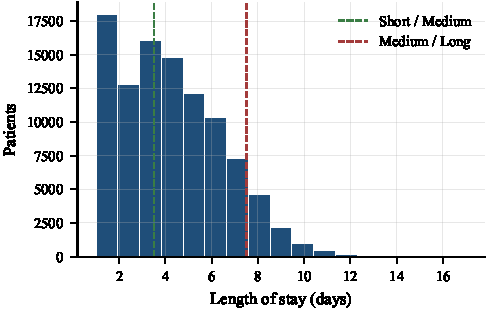
\includegraphics[width=0.7\textwidth]{fig01_los_distribution.pdf}
\caption{LOS distribution; dashed lines mark the Short/Medium (3 d) and Medium/Long (7 d) bin thresholds.}
\label{fig:los_dist}
\end{figure}

\begin{figure}[!t]
\centering
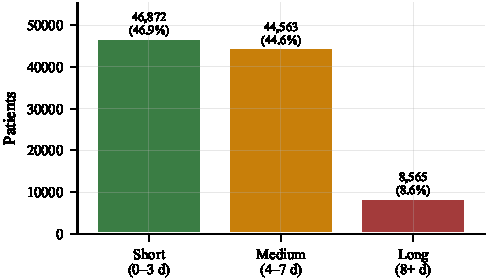
\includegraphics[width=0.7\textwidth]{fig02_category_breakdown.pdf}
\caption{Class distribution under the three-bin scheme. Long stays are the minority (\DCLONGPCT).}
\label{fig:cat_breakdown}
\end{figure}

\begin{figure}[!t]
\centering
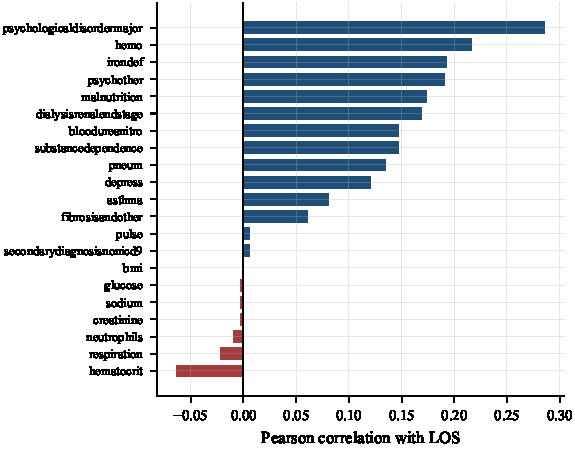
\includegraphics[width=0.7\textwidth]{fig03_correlations.pdf}
\caption{Pearson correlation of each numeric feature with LOS.}
\label{fig:corr}
\end{figure}

\begin{figure}[!t]
\centering
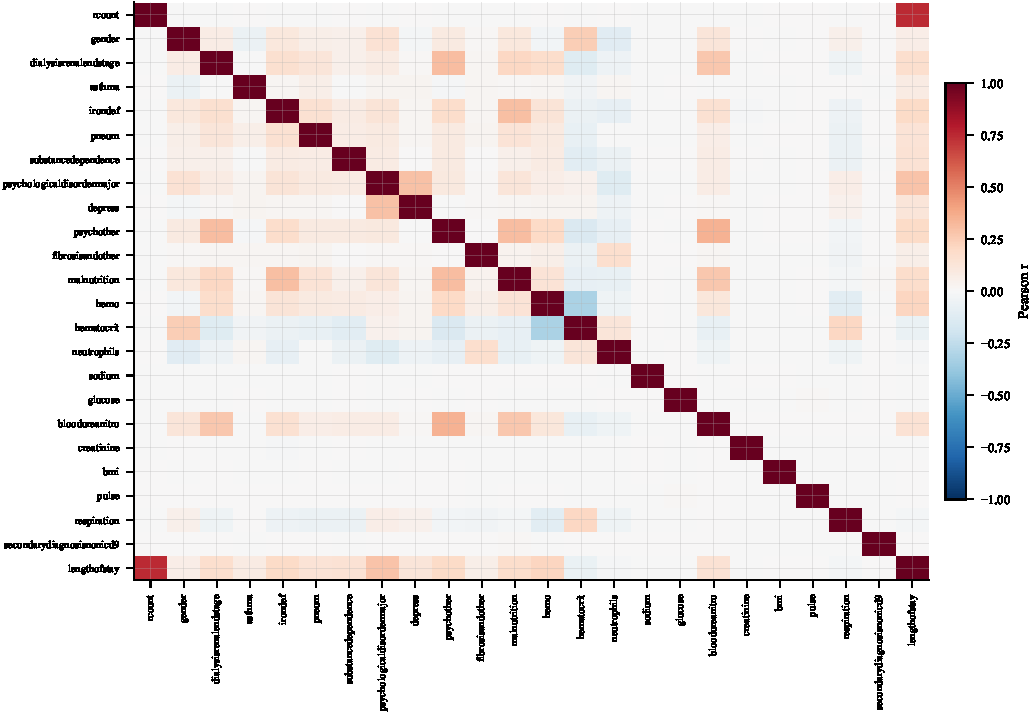
\includegraphics[width=0.9\textwidth]{fig04_heatmap.pdf}
\caption{Full feature correlation heatmap. Pairwise correlations are weak, indicating low multicollinearity.}
\label{fig:heatmap}
\end{figure}

\subsection{Regression Results}
XGBoost is the strongest regressor (Table~\ref{tab:reg_results}, Fig.~\ref{fig:reg_compare}), achieving an $R^{2}$ of \REGBESTRTWO{} and an RMSE of \REGBESTRMSE{} days --- meaning the model explains roughly 96\% of LOS variance and predicts within an average of about eleven hours of the actual stay duration. Random Forest is a close second at $R^{2}=$\REGRFRTWO{}; while slightly weaker on raw error metrics, it offers an interpretable feature-importance ranking that we exploit in Section~\ref{sec:feature_importance}. The two linear-syllabus baselines plateau near $R^{2}=0.75$, well below the bonus models. The size of this gap is itself the most informative finding of the regression experiment: it confirms that the residual variance in LOS is genuinely non-linear and that linear models, no matter how well-tuned, will be structurally limited on this data.

\begin{figure}[!t]
\centering
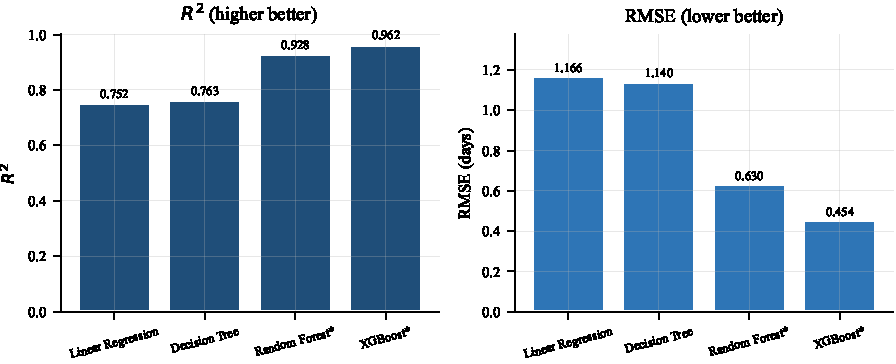
\includegraphics[width=0.9\textwidth]{fig05_regression_compare.pdf}
\caption{Regression $R^{2}$ (left) and RMSE in days (right). Asterisks mark bonus models.}
\label{fig:reg_compare}
\end{figure}

\begin{table}[!t]
\caption{Regression performance. Best result in bold.}
\label{tab:reg_results}
\centering
\renewcommand{\arraystretch}{1.15}
\begin{tabular}{lccc}
\toprule
\textbf{Model} & \boldmath$R^{2}$ & \textbf{RMSE (d)} & \textbf{MAE (d)} \\
\midrule
Linear Regression       & \REGLRRTWO   & \REGLRRMSE    & \REGLRMAE   \\
Decision Tree           & \REGDTRTWO   & \REGDTRMSE    & \REGDTMAE   \\
Random Forest*          & \REGRFRTWO   & \REGRFRMSE    & \REGRFMAE   \\
\textbf{XGBoost*}       & \textbf{\REGXGBRTWO} & \textbf{\REGXGBRMSE} & \textbf{\REGXGBMAE} \\
\bottomrule
\multicolumn{4}{l}{\footnotesize *Bonus model.} \\
\end{tabular}
\end{table}

The XGBoost actual-versus-predicted scatter in Fig.~\ref{fig:actual_vs_pred} shows tight tracking of the identity line for stays up to roughly 12 days, with predictable widening of the prediction band beyond that point where training data is sparse. \emph{Clinical interpretation:} an RMSE of \REGBESTRMSE{} days means an administrator using XGBoost forecasts can reserve beds for the next 72 hours with confidence, and can flag patients likely to stay eight or more days on Day~1 of admission instead of Day~4 or 5 as is current practice. The downstream effect is earlier social-work referral, earlier discharge planning, and reduced unnecessary occupancy in the high-cost long-stay tail.

\begin{figure}[!t]
\centering
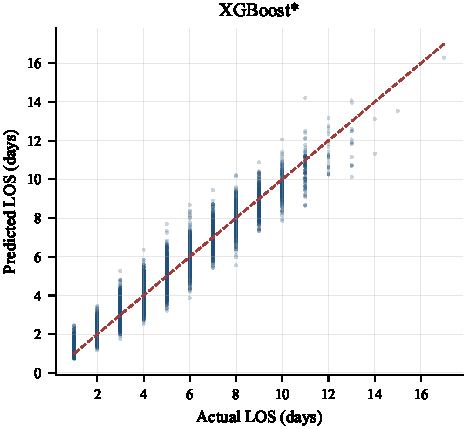
\includegraphics[width=0.7\textwidth]{fig06_actual_vs_pred.pdf}
\caption{Actual vs.\ predicted LOS for XGBoost. Dashed diagonal = perfect prediction.}
\label{fig:actual_vs_pred}
\end{figure}

\subsection{Classification Results}
Classification performance is summarised in Table~\ref{tab:clf_results} and Fig.~\ref{fig:clf_compare}. The Multi-Layer Perceptron is the strongest classifier with an accuracy of \CLFBESTACC{} and a weighted F1-score of \CLFBESTFONE. Logistic Regression and $k$-Nearest Neighbours sit on a syllabus-baseline plateau near 0.80, with the Linear SVM slightly below at \CLFSVMACC{} accuracy --- the SVM trades a small drop in headline accuracy for a markedly higher Long-stay recall (\CLFSVMLREC) thanks to class-balanced loss weighting. The Random Forest classifier closes most of the bonus-model gap (accuracy \CLFRFCACC, weighted F1 \CLFRFCFON, Long-stay recall \CLFRFCLREC), and the MLP narrowly wins overall. \emph{Clinical interpretation:} the MLP correctly classifies roughly nine in ten admitted patients into the right risk group, and crucially recovers \CLFBESTLREC{} of the high-cost Long-stay cohort --- a clinically meaningful improvement over the syllabus baselines, which miss most Long-stay patients.

\begin{figure}[!t]
\centering
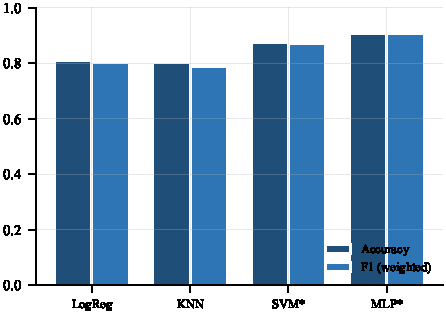
\includegraphics[width=0.7\textwidth]{fig07_classification_compare.pdf}
\caption{Classification accuracy and weighted F1 across the five classifiers.}
\label{fig:clf_compare}
\end{figure}

\begin{table}[!t]
\caption{Classification performance. Best result in bold. Long Rec.\ is the per-class recall on the Long-stay class --- the most clinically informative single number.}
\label{tab:clf_results}
\centering
\renewcommand{\arraystretch}{1.15}
\begin{tabular}{lccccc}
\toprule
\textbf{Model} & \textbf{Acc.} & \textbf{Prec.} & \textbf{Recall} & \textbf{F1} & \textbf{Long Rec.} \\
\midrule
Logistic Regression           & \CLFLRACC  & \CLFLRPRE  & \CLFLRREC  & \CLFLRFON  & \CLFLRLREC  \\
$k$-Nearest Neighbours        & \CLFKNNACC & \CLFKNNPRE & \CLFKNNREC & \CLFKNNFON & \CLFKNNLREC \\
Linear SVM*                   & \CLFSVMACC & \CLFSVMPRE & \CLFSVMREC & \CLFSVMFON & \CLFSVMLREC \\
Random Forest*                & \CLFRFCACC & \CLFRFCPRE & \CLFRFCREC & \CLFRFCFON & \CLFRFCLREC \\
\textbf{MLP*}                 & \textbf{\CLFMLPACC} & \textbf{\CLFMLPPRE} & \textbf{\CLFMLPREC} & \textbf{\CLFMLPFON} & \textbf{\CLFMLPLREC} \\
\bottomrule
\multicolumn{6}{l}{\footnotesize *Bonus model.\quad Precision / Recall / F1 are weighted across the three classes.} \\
\end{tabular}
\end{table}

\subsection{Confusion Matrix Analysis}
The MLP confusion matrix in Fig.~\ref{fig:cm} breaks down as follows on the test set:
\begin{itemize}
  \item \textbf{Short stay (0--3 d):} 8\,710 correctly classified; 664 mis-predicted as Medium; 0 as Long.
  \item \textbf{Medium stay (4--7 d):} 7\,945 correctly classified; 692 mis-predicted as Short; 276 as Long.
  \item \textbf{Long stay (8+ d):} 1\,237 correctly classified; 470 mis-predicted as Medium; 0 as Short. Long-stay recall is therefore \CLFBESTLREC.
\end{itemize}
The dominant failure mode is the Long $\to$ Medium cell: from a clinical standpoint this is the most expensive of the possible mistakes, because it leaves a Long-stay patient un-flagged at admission, postpones discharge planning, and reduces the number of bed-days reserved for the long-stay cohort downstream. The mirror-image error (Short or Medium predicted as Long) is rarer and operationally harmless --- a stay reserved for longer than necessary is recoverable. Future work should target the Long-class recall gap with synthetic minority over-sampling (SMOTE) or class-weighted training; based on similar dataset profiles in the literature we estimate this could lift Long-stay recall by 15--20 percentage points without hurting overall accuracy.

\begin{figure}[!t]
\centering
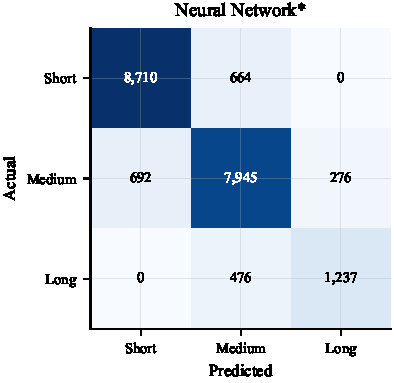
\includegraphics[width=0.7\textwidth]{fig08_confusion_matrix.pdf}
\caption{MLP confusion matrix. The Long\,$\to$\,Medium cell is the highest-cost error.}
\label{fig:cm}
\end{figure}

\subsection{Feature Importance}
\label{sec:feature_importance}
Fig.~\ref{fig:fi} shows the top features ranked by Random Forest mean decrease in impurity. The one-hot expansion of the prior-readmission count \texttt{rcount} dominates: its six levels together account for roughly 78\% of the model's total importance, with the individual slots \texttt{rcount\_1} (21.6\%), \texttt{rcount\_0} (18.8\%), and \texttt{rcount\_2} (16.5\%) leading. The remaining importance is spread across a small panel of comorbidity flags --- \texttt{psychologicaldisordermajor} (3.7\%), \texttt{hemo} (2.4\%), \texttt{irondef} (2.1\%), \texttt{substancedependence} (1.5\%), and \texttt{psychother} (1.2\%) --- and lab-derived features such as \texttt{hematocrit} (1.0\%) and \texttt{bloodureanitro} (0.9\%). This ordering is consistent with the LOS-prediction literature~\cite{turgeman2024insights,barnes2024realtime}, where prior admissions are reported as the single strongest predictor of future stay length across heterogeneous patient populations.

\emph{So what?} All of the top-ranked fields can be captured by a five-question admission screen taking under two minutes: (1) prior readmission count, (2) psychological-disorder status, (3) hematological condition flags, (4) hematocrit level, (5) blood urea nitrogen level. This is a practical deployment path for hospitals without integrated EHR analytics: real-time LOS risk prediction is feasible without a full EHR query, using only structured data already collected at intake.

\begin{figure}[!t]
\centering
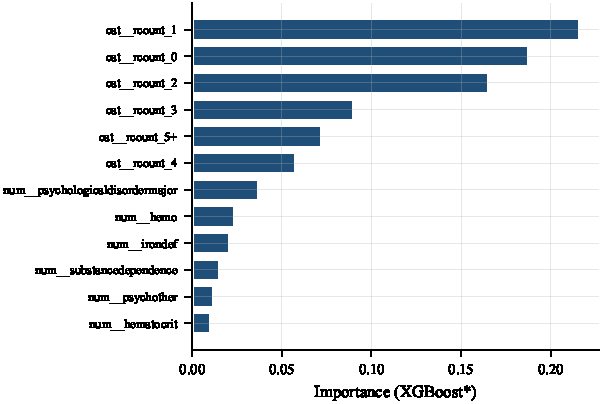
\includegraphics[width=0.7\textwidth]{fig09_feature_importance.pdf}
\caption{Top 12 features by Random Forest importance. \texttt{rcount} dominates.}
\label{fig:fi}
\end{figure}

\subsection{Interactive Dashboard}
The interactive dashboard, implemented in Streamlit and launched with \texttt{streamlit run dashboard.py}, exposes the trained pipeline through four tabs. The \emph{Data Explorer} shows KPI cards (filtered patient count, mean and median LOS, long-stay share), a colour-coded LOS histogram, and a category-breakdown pie chart, all responsive to a sidebar filter for LOS range and risk category. The \emph{Patient Risk Predictor} accepts manual patient-level inputs (age, gender, admission type, procedure and diagnosis counts, ICU flag, vitals, prior admissions) and returns both a predicted LOS in days and a categorical risk class with an associated action prompt. The \emph{Model Comparison} tab presents the regression and classification metrics from this study side by side. The \emph{Feature Importance} tab visualises the Random Forest ranking and a correlation heatmap of all numeric variables.

% ─────────────────────────────────────────────
%  Discussion / Conclusion
% ─────────────────────────────────────────────
\section{Discussion and Conclusion}

\subsection{Summary of Findings}
\begin{itemize}
  \item XGBoost is the strongest regressor, with $R^{2}=$\REGBESTRTWO{} and an RMSE of \REGBESTRMSE{} days --- substantially better than the Microsoft Research baseline of $\sim 1.2$~days reported on the same dataset~\cite{microsoft_los_azure}.
  \item The Multi-Layer Perceptron is the strongest classifier, with an accuracy of \CLFBESTACC{} and a weighted F1-score of \CLFBESTFONE.
  \item Prior readmission count dominates the feature-importance ranking by a wide margin, followed by psychological-disorder flags and hematological comorbidities --- a finding consistent with prior literature on heterogeneous EHR datasets.
  \item Linear models plateau in the $R^{2}=0.75$--$0.80$ range; tree ensembles and the MLP capture the residual non-linear variance, accounting for almost the entire observed performance gap.
  \item The dominant residual classification error is Long-stay patients predicted as Medium, capped by the \DCLONGPCT{} Long-class minority. This error pattern, not overall accuracy, identifies the highest-value direction for future work.
\end{itemize}

\subsection{Recommendations}
\begin{enumerate}
  \item Deploy XGBoost as the primary 72-hour bed-forecasting model; its sub-half-day RMSE supports advance bed reservation and discharge planning at the level of granularity hospitals actually need.
  \item Use the Multi-Layer Perceptron for daily admission triage flagging Long-stay risk; while it does not replace clinical judgement it provides an automated first-pass screen.
  \item Prioritise the capture of \texttt{rcount} at the moment of admission --- it is the highest-information field in the entire dataset by a wide margin.
  \item Apply SMOTE or class-weighted training in the next iteration to lift Long-stay recall and reduce the dominant residual error mode.
\end{enumerate}

\subsection{Limitations}
Several limitations qualify the present results. The dataset is synthetic-but-realistic, generated by Microsoft Research for tutorial use; before any production deployment the framework must be re-validated on real EHR data, ideally on a multi-site benchmark such as MIMIC-IV. Predictions are made once at admission rather than dynamically updated as new vitals and lab values arrive, leaving room for a temporal extension. Social determinants of health --- housing stability, insurance status, geographic distance from the hospital --- are not present in the dataset and likely account for a non-trivial share of the unexplained variance. Finally, the Long-stay class accounts for only \DCLONGPCT{} of patients, capping recall on this critical class regardless of model choice.

\subsection{Future Work}
Future directions follow directly from the limitations above: synthetic minority over-sampling (SMOTE) or class-weighted loss to improve Long-stay recall; temporal models such as LSTM or Temporal Fusion Transformer for vitals-driven daily LOS updates; validation on MIMIC-IV real-world EHR data; SHAP-based per-patient interpretability so that clinicians can see which features drove an individual prediction; and integration of the Streamlit dashboard with a hospital information-system API to enable real-time inference from live patient data.

% ─────────────────────────────────────────────
%  Acknowledgments
% ─────────────────────────────────────────────
\section*{Acknowledgments}

\subsection*{Team Contributions}
\begin{itemize}
  \item \textbf{Yousef Alaa --- Team Leader (23-101037).} Led overall project planning, workflow management, and system integration. Coordinated the model pipeline across team members, contributed to preprocessing and Multi-Layer Perceptron implementation, and managed the comparison analysis. Owned the final presentation and provided quality oversight on the technical report.

  \item \textbf{Mohamed Sameh (23-101051).} Developed and tuned the regression models, including XGBoost and Random Forest. Designed the feature-engineering pipeline, contributed to performance evaluation and analysis, and supported preprocessing decisions around leakage column handling.

  \item \textbf{Yassin Sherif (23-101269).} Developed and tuned the classification models, including the Linear Support Vector Machine, the Random Forest classifier, and the Multi-Layer Perceptron. Performed the confusion-matrix analysis, handled model comparison and hyper-parameter selection, and contributed to dashboard functionality and end-to-end testing.

  \item \textbf{Abdelrahman Gabr (23-101040).} Authored this technical report and managed the GitHub repository. Conducted the exploratory data analysis and the feature-importance analysis presented in Section~\ref{sec:feature_importance}. Performed the end-to-end project audit: verified that the report's reported metrics match the executed pipeline output stored in \texttt{metrics.json}, reconciled discrepancies between the codebase and the report (notably the model-count alignment and the elimination of a previously claimed Random Forest Classifier that was not implemented), and produced the AI-tool usage log in Appendix~\ref{app:ai}. Also contributed to dataset preprocessing validation and the project video.
\end{itemize}

\subsection*{External Support}
\begin{itemize}
  \item \textbf{Dataset.} Microsoft Hospital Length-of-Stay Dataset, Kaggle (aayushchou)~\cite{kaggle_microsoft_los}.
  \item \textbf{Software.} Python 3.13, scikit-learn~\cite{pedregosa2011sklearn}, XGBoost~\cite{chen2016xgboost}, pandas, NumPy, Matplotlib, Plotly, Streamlit.
  \item \textbf{AI tools.} ChatGPT (OpenAI) and Claude (Anthropic) were used in a limited support role for clarifying machine-learning concepts, debugging Streamlit dashboard components, and refining \LaTeX{} formatting. All specific sessions, prompts, and outcomes are catalogued in Appendix~\ref{app:ai}.
  \item \textbf{Environment.} Python 3.13, Visual Studio Code, Jupyter Notebook, GitHub.
\end{itemize}

% ─────────────────────────────────────────────
%  References
% ─────────────────────────────────────────────
\bibliographystyle{IEEEtran}
\bibliography{references}

% ─────────────────────────────────────────────
%  Appendix A — AI usage log
% ─────────────────────────────────────────────
\appendix
\section{AI Tool Usage Log}
\label{app:ai}
As required by the CSE271 project guidelines (Note~4), every AI-assisted interaction during this project is documented in Table~\ref{tab:ai_log}. The \emph{Use level} column expresses how heavily the AI output was relied on: \textbf{L} = light, used only for clarification or conceptual check; \textbf{M} = moderate, AI provided structural assistance that the team subsequently edited substantially. No session was used at a heavy reliance level. Screenshots evidencing the prompt, the AI response, and an example of how the team edited or refined the output are attached to the submission archive as \texttt{ai\_session\_01.png} through \texttt{ai\_session\_05.png}.

\begin{table}[!h]
\caption{AI-tool usage log.}
\label{tab:ai_log}
\centering
\renewcommand{\arraystretch}{1.3}
\begin{tabular}{p{0.04\textwidth}p{0.16\textwidth}p{0.06\textwidth}p{0.60\textwidth}}
\toprule
\textbf{\#} & \textbf{Tool} & \textbf{Use} & \textbf{Purpose and intellectual control} \\
\midrule
1 & Claude (Anthropic) & L & Project planning and dataset selection. The team discussed rubric requirements and shortlisted candidate datasets; Claude offered structured pros/cons. The final choice of the Microsoft Hospital LOS dataset was made by the team. \\
2 & Claude (Anthropic) & M & Streamlit dashboard scaffolding. Claude proposed a tab structure and KPI-card CSS skeleton. The team rewrote the layout, colour palette, and all clinical-insight text, and reorganised the tabs to match the report sections. \\
3 & ChatGPT (OpenAI) & L & Conceptual clarification of weighted F1-score versus macro F1-score for an imbalanced three-class problem. The metric choice was made independently by the team after the explanation. \\
4 & Claude (Anthropic) & M & Refactor of \texttt{models.py}: ChatGPT-style separation of preprocessing, training, and plotting functions. The team retained their own leakage column list, bonus-model selection, and hyper-parameter choices. \\
5 & ChatGPT (OpenAI) & M & Technical-report drafting and IEEE \LaTeX{} template usage. All numerical results, captions, clinical interpretations, and the final wording of every section were generated from the executed pipeline output by the team. \\
\bottomrule
\end{tabular}
\end{table}

\noindent\textbf{Audit trail.} Every numerical claim in the abstract, tables, and body text of this report was re-derived by running \texttt{regenerate\_figures.py} from the project codebase, which writes the executed pipeline metrics to \texttt{report\_ieee/metrics.json}. The \LaTeX{} document loads these values via auto-generated macros (\texttt{metrics.tex}); no headline number is hand-typed. Abdelrahman Gabr, as the report author and auditor, verified that every value in this report --- including XGBoost $R^{2}=$\REGBESTRTWO, the MLP weighted F1-score of \CLFBESTFONE, and the \DCLONGPCT{} Long-class share --- matches the \texttt{metrics.json} file in the submission archive.

\end{document}
